%!TEX root = ../../main.tex

\section{Theoretische Grundlage}

\subsection{Haskell}
\setLayout{mainpoint}
\begin{frame}{}
    \frametitle{Haskell}
\end{frame}

\setLayout{vertical}
\begin{frame}{}

    \footnotesize

    \begin{block}{Haskell}
        Haskell ist eine nicht strenge, rein funktionale Sprache mit statischer Typisierung und algebraischen Datentypen. Es ist eine reichhaltige Sprache, die nützliche Funktionen wie Currying, Infix-Präfix-Operationen, anonyme Funktionen und Listenverständnis, Monaden, bietet \cite{history-of-haskell}.

    \end{block}

    \begin{block}{Typsystem-Erweiterungen}
    die Sprache enthält Typsystem-Erweiterungen wie polymorphe Rekursion, höherwertige Quantifizierung, höherrangige Typen, lexikalisch beschränkte Typvariablen, generische Programmierung, Template-Meta-Programmierung und vieles mehr \cite{history-of-haskell} 
    \end{block}

    \begin{alertblock}{Haskell ist schön}
        Viele Entwickler behaupten, dass Haskell-Programme schön aussehen. 
        \cite{history-of-haskell} 
    \end{alertblock}

\end{frame}


\subsection{GraphQL}
\setLayout{mainpoint}
% \setBGColor{UHHRed}
\begin{frame}{}
    \frametitle{GraphQL}
\end{frame}


\setLayout{vertical}
\begin{frame}{}

    \footnotesize

    \begin{block}{Was ist GraphQL?}
        GraphQL ist ein Anwendungsschicht-Framework zur Lösung der Effizienzprobleme der Kommunikation \cite{gql-iot}.         
    \end{block}

    \begin{block}{von Facebook Entwicklt}
        Es wurde drei Jahre lang intern bei Facebook entwickelt und seine Spezifikation und seine Referenzimplementierung 2016 veröffentlicht.
        \cite{initial-analysis-of-gql}
    \end{block}

    \begin{block}{GraphQL als aktueller Trend}
        Seit ihrem ersten Erscheinen hat sie ein reiches Open-Source-Ökosystem und das Vertrauen von Unternehmen aus verschiedenen Sektoren gewonnen. z.B: (GitHub), Unterhaltung (Netflix), Finanzen (PayPal), Reisen (KLM), etc \cite{morph-gql-1,gql-healthcare}.
    \end{block}

\end{frame}


\section{Morpheus GraphQL}
\setBGColor{white}
\begin{frame}{Morpheus GraphQL}
    \begin{figure}
        \centering
        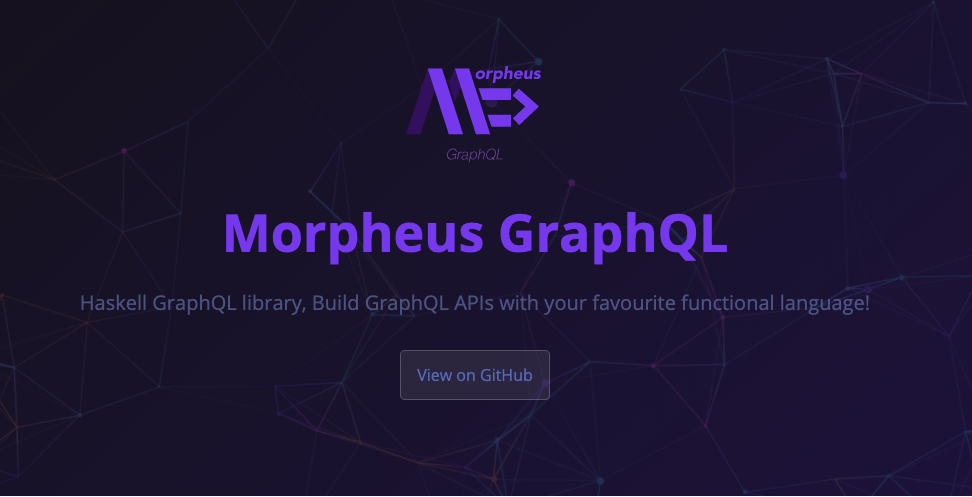
\includegraphics[width=1.1\textwidth]{assets/img/morpheus-graphql-bg.png}
    \end{figure}
\end{frame}